\section{问题四：含收缩动边界的烘干时长模型}
\label{sec:p4}

\subsection{相对问题三的增量}

问题四相对问题三只增加两件事。其一，物性闭合换成附录 4，

\begin{align}
\rho(C)&=760+90C, &
c_p(C)&=1850+2150\,\frac{C}{C+1},
\label{eq:app4_rho_cp}\\
k(C)&=0.12+0.20\,\frac{C}{C+1}, &
D(C,T)&=4.2\times10^{-4}\,\mathrm{e}^{-0.30/C}\,\mathrm{e}^{-3850/T_K}.
\label{eq:app4_k_D}
\end{align}

其二，外半径由固定值改为附件 2 给出的实测时程。题面“请根据附件 2”
意味着收缩是给定的运动学数据而非待求量，因此模型不需要补充任何收缩本构，
也不应由含水率反推半径。附件 2 覆盖 $0$ 至 $259200$ s、间隔 $1800$ s 共
$145$ 个点，中间时刻按线性插值取用。

式~\eqref{eq:app4_k_D}~与附录 3 的关键差别在扩散系数：
同一状态 $C=2.55$、$T=28$ °C 下附录 4 给出 $1.0471\times10^{-9}$ m$^2$/s，
比附录 3 的 $5.6417\times10^{-9}$ 小 $5.4$ 倍。热扩散率也更小，
由附录 3 的 $1.4483\times10^{-7}$ 降到 $7.8501\times10^{-8}$ m$^2$/s。
两项都指向更慢的输运。

第~\ref{sec:model}~节的干质量坐标使动边界不需要任何额外处理：
收缩只通过式~\eqref{eq:mass_s}~的系数 $4/R(t)^2$ 与式~\eqref{eq:bc_s}~的
表面通量系数进入方程组，两者都是已知的时间函数，
求解域恒为 $[0,1]$，与问题三共用同一求解器。

判据的取法与问题三一致，只是达标区间随边界一起收缩，本问的目标函数与约束为

\begin{equation}
\begin{aligned}
&\min_{t>0}\ \ J_4(t)=t,\\
&\mathrm{s.t.}\ \ g_4(t)\equiv\max_{0\le r\le R(t)}C(r,t)-C_{\mathrm{th}}<0,
\qquad C_{\mathrm{th}}=0.15~\text{kg/kg},\\
&\phantom{\mathrm{s.t.}}\ \ R(t)=\mathrm{interp}\bigl(t;\{(t_i,R_i)\}_{i=1}^{145}\bigr),
\qquad R(0)=R_0 .
\end{aligned}
\label{eq:p4_obj}
\end{equation}

式~\eqref{eq:p4_obj}~与式~\eqref{eq:p3_obj}~的差别仅在两处约束。
其一，含水率场改由附录 4 的物性闭合确定，
即以式~\eqref{eq:app4_rho_cp} 与 \eqref{eq:app4_k_D} 的系数，
代入式~\eqref{eq:mass_s} 至 \eqref{eq:bc_s} 求解；
其二，几何约束由 $R\equiv R_0$ 换成附件 2 的实测半径时程 $R(t)$，
$\mathrm{interp}$ 表示在 $145$ 个实测点之间线性插值。
$R(t)$ 是给定的运动学输入而非决策变量，因此目标函数 $J_4(t)=t$
的最优值同样是一个由正演决定的首达时刻，不含任何可调自由度。
求解域取到 $R(t)$ 而非 $R_0$，意味着 $t$ 时刻已收缩到药材之外的位置
不参与达标判定，这也是表~\ref{tab:q4_C}~末列改用“药材表面”的原因。

\subsection{收缩数据的形态}

前 $6$ h 已完成总收缩量的 $78.1\%$，半径由 $2.000$ cm 降至 $1.374$ cm；完整收缩曲线及其对扩散尺度的解释见附录 B。
\iffalse

\begin{figure}[!htbp]
  \centering
  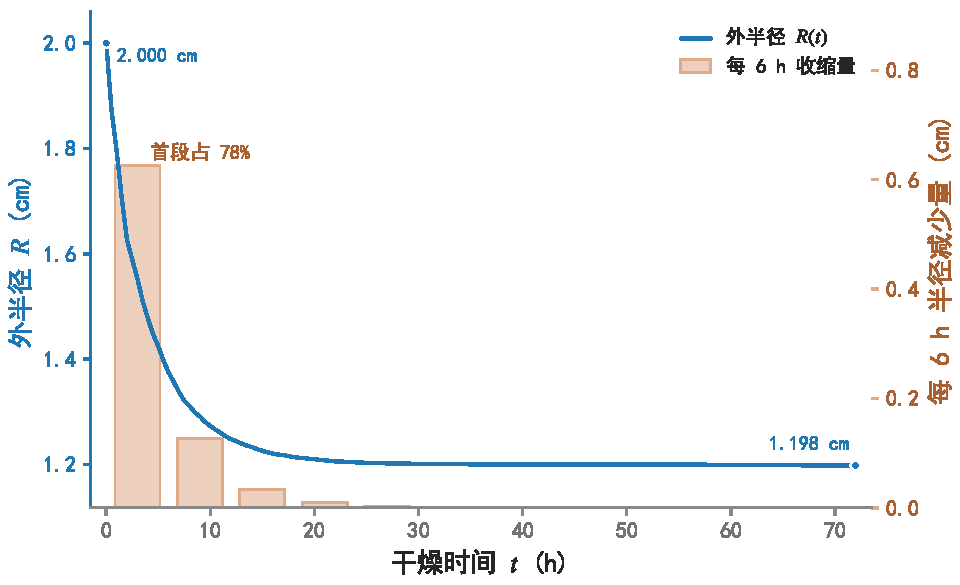
\includegraphics[width=0.9\textwidth,height=0.8\textheight,keepaspectratio]{../figures/fig_shrinkage_curve.pdf}
  \caption{药材半径收缩曲线}
  \label{fig:shrinkage_curve}
\end{figure}

收缩几乎全部发生在烘干初期（图~\ref{fig:shrinkage_curve}~给出附件 2 全部
$145$ 个点的半径时程与每 $6$ h 的收缩增量）。半径由 $2.000$ cm 单调降到 $1.198$ cm，
横截面积仅剩初始的 $35.88\%$。收缩的时间分布极不均匀：
前 $6$ h 内半径就下降 $0.626$ cm，占全程总收缩量的 $78.1\%$；
到 $12$ h 累计完成 $93.8\%$；$36$ h 之后半径几乎冻结在 $1.200$ cm。

这一形态决定了收缩的作用不容小视。前 $6$ h 正是含水率梯度最陡、
传质最活跃的时段，扩散路程恰在最关键的阶段被缩短 $31.3\%$。
由式~\eqref{eq:mass_s}，半径由 $2.000$ cm 降到 $1.374$ cm 使系数 $4/R^2$
放大到 $2.12$ 倍，收缩到最小半径 $1.198$ cm 时更达 $2.79$ 倍，
等效于扩散被显著加速。

\fi
\subsection{结果}

按 $N=160$、$\Delta t=1$ s 推进到第 $183\,900$ 步（即 $51.0833$ h）时判据首次满足，
与问题三同法插值得

\begin{equation}
t_{\mathrm{dry}}=51.0711~\text{h}=2.1280~\text{d}.
\label{eq:tdry_q4}
\end{equation}

末输出步 $\max_rC=0.149977$ 已低于阈值、前一步 $0.150008$ 仍高于阈值，
确为首次穿越；全程守恒残差 $1.547\times10^{-10}$。
网格无关性上，$N=48$、$112$、$160$ 分别给出 $51.042455$、$51.067066$、
$51.071110$ h，相邻相对差 $4.819\times10^{-4}$ 与 $7.919\times10^{-5}$，
末组远优于判据，对应图~\ref{fig:grid_convergence}~的第二条曲线。

与式~\eqref{eq:tdry_q3}~同理，式~\eqref{eq:tdry_q4}~也是条件式结论：
附件 1 实测只覆盖前 $4$ h，占本问总时长的 $7.8\%$，
其余 $92.2\%$ 的时间轴由平台均值常数延拓段提供边界条件，
第~\ref{sec:validation}~节给出的 $\pm0.5$ °C 扰动对应约 $\mp1.6\%$ 的时长变化。
问题四还多一重不确定度来源：半径时程是最灵敏的输入，
半径弹性达 $1.810$，故式~\eqref{eq:tdry_q4}~应理解为
“在恒温平台条件持续保持、且附件 2 半径数据准确的前提下”的烘干时长。

\begin{figure}[!htbp]
  \centering
  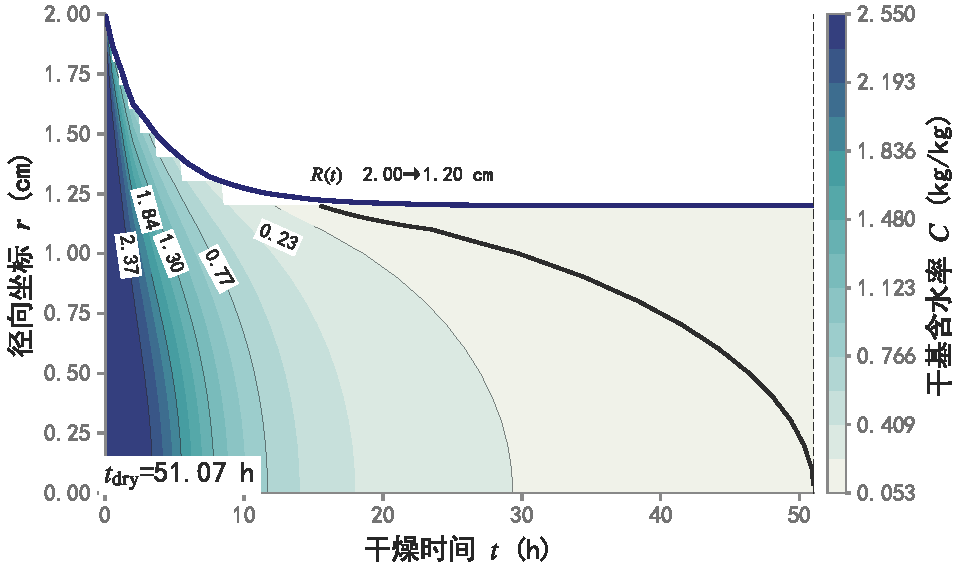
\includegraphics[width=0.74\textwidth,height=0.42\textheight,keepaspectratio]{../figures/fig_q4_field_C_moving.pdf}
  \caption{问题四移动边界含水率场}
  \label{fig:q4_field_C_moving}
\end{figure}

移动边界在前 $6$ h 迅速内收、随后趋于水平，
而含水率等值线始终与边界保持相似的排布
（图~\ref{fig:q4_field_C_moving}~在含水率场上叠加 $R(t)$ 曲线，域外区域留白）。
等值线与边界的这种相似排布，是仿射收缩假设下每个 $s$ 值
标记同一批干物质的直观体现。留白区域并非缺失数据，
而是该时刻药材已经收缩到那个半径之内，物理上不存在的位置不做插值编造。

\begin{table}[H]
  \centering
  \caption{问题四烘干过程的水分浓度（kg/kg）}
  \label{tab:q4_C}
  \setlength{\tabcolsep}{4pt}
  \begin{tabular}{ccccccc}
  \toprule
  时间 (h) & $R(t)$ (cm) & $r=0$ cm & $r=0.5$ cm & $r=1.0$ cm & 药材表面 & $\bar C$ \\
  \midrule
  6  & 1.3740 & 1.7195 & 1.5376 & 1.0226 & 0.4208 & 1.0652 \\
  12 & 1.2480 & 0.7375 & 0.6545 & 0.4082 & 0.1669 & 0.4760 \\
  18 & 1.2140 & 0.4086 & 0.3686 & 0.2397 & 0.0892 & 0.2803 \\
  24 & 1.2040 & 0.2850 & 0.2610 & 0.1789 & 0.0673 & 0.2054 \\
  30 & 1.2010 & 0.2263 & 0.2093 & 0.1492 & 0.0595 & 0.1685 \\
  36 & 1.2000 & 0.1928 & 0.1796 & 0.1316 & 0.0559 & 0.1469 \\
  42 & 1.2000 & 0.1712 & 0.1603 & 0.1199 & 0.0541 & 0.1327 \\
  48 & 1.2000 & 0.1561 & 0.1468 & 0.1115 & 0.0530 & 0.1225 \\
  烘干结束 51.0711 & 1.2000 & 0.1500 & 0.1413 & 0.1081 & 0.0526 & 0.1184 \\
  \bottomrule
  \end{tabular}
\end{table}

表~\ref{tab:q4_C}~的列式与问题三不同，末列为药材表面处的数值，
这是题面明确要求的格式，也是收缩问题下唯一自洽的写法：
$t\ge6$ h 时 $R(t)<1.5$ cm，$r=1.5$ cm 与 $r=2.0$ cm 两个位置
已经在药材之外，硬套问题三的固定半径列会得到没有物理意义的数值。
每隔 $60$ s、每隔 $0.1$ cm 的完整结果见 \verb|result4.xlsx|，
共 $3065$ 行 $\times$ $23$ 列：按第~\ref{sec:p1}~节说明的列数计法，
即一列时间标签加 $0$ 至 $2.0$ cm 共 $21$ 个半径列，再加“药材表面”末列。
超出当时 $R(t)$ 的位置留空，共 $23\,157$ 个空单元，
占 $21$ 个半径列的 $36.0\%$，不做域外插值。
若只关心全程始终有值的部分，$0$ 至 $1.1$ cm 的子集在整个烘干过程中
都位于药材内部，因为最小半径为 $1.198$ cm。

\subsection{消融实验：两个反向机制的分解}

式~\eqref{eq:tdry_q4}~比式~\eqref{eq:tdry_q3}~只短 $11.0\%$。
若就此结论“收缩影响有限”，会得到完全错误的物理图像，
因为问题四同时改动了物性与几何，而两者作用方向相反。
为把它们分开，本文按 $2\times2$ 设计做四次独立重算，
在 $N=112$、$\Delta t=1$ s 下统一比较。

\begin{table}[H]
  \centering
  \caption{物性与收缩的消融实验}
  \label{tab:ablation}
  \begin{tabular}{cccc}
  \toprule
  组合 & 物性闭合 & 几何 & $t_{\mathrm{dry}}$ (h) \\
  \midrule
  基准（问题三） & 附录 3 & $R\equiv R_0$ & 57.4040 \\
  仅换物性       & 附录 4 & $R\equiv R_0$ & 129.7587 \\
  仅加收缩       & 附录 3 & $R(t)$        & 25.2269 \\
  问题四（全）   & 附录 4 & $R(t)$        & 51.0671 \\
  \bottomrule
  \end{tabular}
\end{table}

两个主效应都很强且符号相反（表~\ref{tab:ablation}）。以下百分比一律以
该表首行的基准 $t_{\mathrm{base}}=57.4040$ h 为分母：
单换附录 4 使烘干时长增加 $126.0\%$（$+72.3547$ h），因为扩散系数小 $5.4$ 倍；
单加收缩使烘干时长减少 $56.1\%$（$-32.1771$ h），因为扩散路程被大幅缩短。
两者相加应为 $+40.1775$ h，而实测总变化只有 $-6.3370$ h，
交互项因此为

\begin{equation}
\Delta_{\mathrm{int}}
=t_{\mathrm{both}}-t_{\mathrm{base}}
-\left(t_{\mathrm{prop}}-t_{\mathrm{base}}\right)
-\left(t_{\mathrm{shrink}}-t_{\mathrm{base}}\right)
=-46.5145~\text{h}.
\label{eq:interaction}
\end{equation}

\iffalse
\begin{figure}[!htbp]
  \centering
  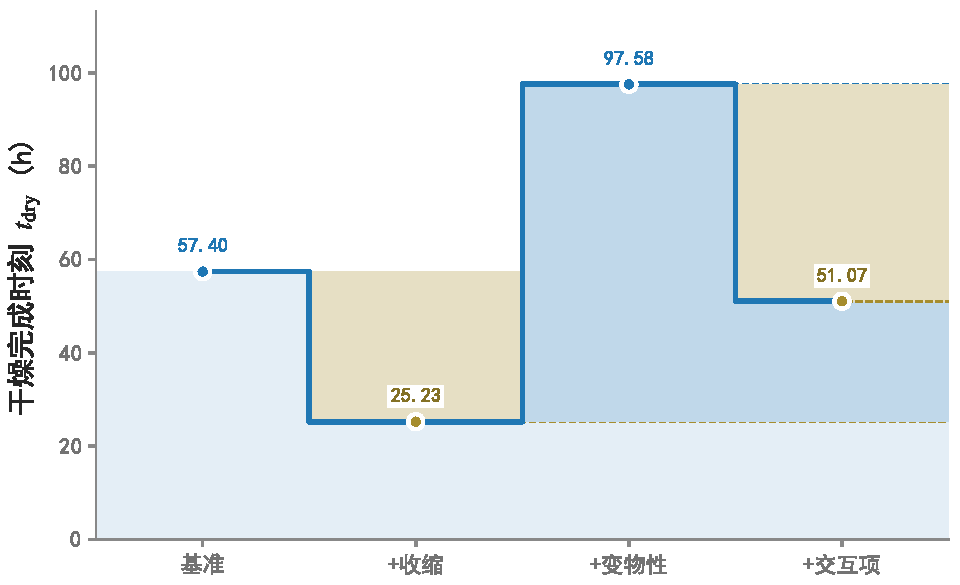
\includegraphics[width=0.9\textwidth,height=0.8\textheight,keepaspectratio]{../figures/fig_q4_ablation.pdf}
  \caption{收缩与物性的加性分解}
  \label{fig:q4_ablation}
\end{figure}

$+72.3547$ h 的物性效应、$-32.1771$ h 的收缩效应与 $-46.5145$ h 的交互项
合成最终的 $-6.3370$ h，瀑布图逐段给出这一累加过程
（图~\ref{fig:q4_ablation}）。交互项的量级与两个主效应相当，
说明两因素强耦合、不可线性叠加——收缩缩短路程的收益在扩散更慢的
附录 4 闭合下被进一步放大。

由此得到本问最重要的定性结论：收缩是本题最强的单一机制，
单独作用可把烘干时长压缩过半，只是在问题四中被附录 4 慢 $5.4$ 倍的扩散
大部分抵消，表面上才呈现为 $-11.0\%$ 的温和变化。
只报告净变化会掩盖这一事实。
\fi

\subsection{收缩数据与物性公式的一致性核查}

附件 2 的实测半径与附录 4 密度闭合在均质混合物假设下不相容：由半径反演的平均含水率自 $24$ h 起为负。本文因此以题目明确要求使用的实测半径为准；完整反演与讨论见附录 C。
\iffalse

附件 2 的实测半径与附录 4 的密度公式描述的是否同一件事，需要独立核查。
干质量线密度

\begin{equation}
\frac{M_s}{\pi L}=\frac{\rho_4(C_0)R_0^{2}}{1+C_0}=0.111493~\text{kg/m}
\label{eq:dry_linear}
\end{equation}

全程恒定。若认为整根药材的湿质量由附录 4 的 $\rho=760+90\bar C$ 描述，
则由实测半径可反演平均含水率：

\begin{equation}
\bar C_{\mathrm{vol}}(t)=\frac{0.111493-760R(t)^{2}}{90R(t)^{2}-0.111493}.
\label{eq:inversion}
\end{equation}

代入附件 2 的半径，$\bar C_{\mathrm{vol}}$ 在 $0$、$6$、$12$、$18$ h 处
分别为 $2.5500$、$0.3385$、$0.0706$、$0.0052$，自 $24$ h 起变为
$-0.0134$ 并继续下降到 $72$ h 的 $-0.0245$。含水率为负在物理上不可能，
说明这两处题设不能同时成立。

改用体积可加性闭合作对照，取 $\kappa=\rho_s/\rho_w=760/1000=0.7600$，
由 $V/V_0=(1+\kappa\bar C)/(1+\kappa C_0)$ 反演得 $\bar C(18~\text{h})=0.1086$，
而输运模型在同一时刻给出 $0.2803$，两者偏离 $61.3\%$。
两条路径在同一时刻相差如此之大，表明在“整根药材为均质两相混合物”这一
闭合假设下，附件 2 的收缩数据与附录 4 的物性公式不相容。
该结论依赖上述闭合假设，不能推广为两组数据本身必有一组错误。

这一矛盾无法在题设范围内消除，本文的处理是以附件 2 的实测半径为准，
理由有两条：题面明确要求“根据附件 2”确定烘干时长，实测数据的地位高于
由密度公式反推的间接量；且反演路径本身依赖“整根药材为均质两相混合物”
这一比输运模型更强的额外假设。同时必须承认这是问题四结果不确定度的
主要来源——第~\ref{sec:validation}~节的灵敏度分析显示 $R(t)$ 是全部参数中
最灵敏的一项，半径弹性达 $1.810$，故式~\eqref{eq:tdry_q4}~的可靠性
主要取决于附件 2 数据本身的可靠性。
\fi
